% MSDM5054 Final Project report (NeurIPS style, <= 8 pages of content).
% On Overleaf: add neurips_2019.sty (handout link) next to this file; it is then used automatically.
% Without it, the layout below reproduces the NeurIPS text block (5.5in x 9in, Times, 10pt).
\documentclass[10pt]{article}
\makeatletter
\IfFileExists{neurips_2019.sty}{\usepackage[final]{neurips_2019}}{%
  \usepackage[letterpaper,textwidth=5.5in,textheight=9in,top=1in,headsep=0pt,headheight=0pt]{geometry}%
  \usepackage{times}%
  \renewcommand{\@maketitle}{\begin{center}{\Large\bfseries\@title\par}\vskip 1em{\@author\par}\end{center}\vskip 1em}}
\makeatother
\usepackage[utf8]{inputenc}
\usepackage[T1]{fontenc}
\usepackage{hyperref,url,booktabs,amsmath,amssymb,nicefrac,microtype,graphicx,xcolor}
\usepackage[font=small,labelfont=bf,skip=4pt]{caption}
\usepackage{subcaption}
\setlength{\textfloatsep}{10pt plus 2pt minus 2pt}
\setlength{\floatsep}{8pt plus 2pt minus 2pt}

\title{What Do Machines Learn About Expected Returns?\\A Replication of \emph{Empirical Asset Pricing via Machine Learning}}

\author{%
  Zhang Qi \qquad Wei Fanjing \qquad Tang Yunshu \qquad Du Yunhe\\
  MSDM5054 Statistical Machine Learning, The Hong Kong University of Science and Technology\\
  \texttt{Code: \url{https://github.com/ZQ-77777/gkx-replication}}
}

\begin{document}
\maketitle

\begin{abstract}
We replicate Gu, Kelly and Xiu (GKX, 2020), who compare machine-learning methods for predicting monthly excess returns of
U.S.\ stocks from 94 firm characteristics, 8 macroeconomic predictors and 74 industry dummies (920 inputs). Using the
authors' public characteristics and GKX's recursive scheme (annual refits, expanding training window, rolling 12-year
validation window, 30 out-of-sample years 1987--2016), we estimate 14 specifications: OLS and OLS-3 with and without Huber
loss, elastic net, PCR, PLS, random forest, gradient-boosted trees and neural networks NN1--NN5. Regularised, reduced-rank
and nonlinear models all predict out of sample (monthly $R^2_{oos}$ of 0.07--0.34\%), with the best result from the
shallow network NN1 (0.34\%, GKX: 0.33\%), whereas OLS with all 920 inputs fails badly ($-23.5\%$ with Huber loss,
GKX: $-3.46\%$). Two findings go beyond a numerical replication. First, the way macroeconomic information enters matters:
tree models that see macro predictors as standalone levels forecast the market-wide return component and lose out of sample.
Second, the dominant predictors are price trends, liquidity and volatility, in line with GKX, while statistical separation
between the better models is weaker than in the paper.
\end{abstract}

% =====================================================================
\section{Introduction}
The conditional expected return of a stock -- its risk premium -- is the central object of empirical asset pricing, and it
is hard to measure: monthly returns are dominated by unpredictable news, hundreds of candidate predictors have been
proposed, and their effects may be nonlinear and depend on the economic environment. GKX~\cite{gkx} cast the problem as
prediction, $r_{i,t+1}=g^\star(z_{i,t})+\varepsilon_{i,t+1}$, and ask which machine-learning methods approximate $g^\star$
best. We replicate their main analysis and organise the report around five questions:

\textbf{Q1} Do we reproduce the out-of-sample ranking of GKX Table~1?
\textbf{Q2} Why does OLS with many predictors fail, and how much do robust loss, regularisation and dimension reduction help?
\textbf{Q3} What do nonlinear models (trees, networks) add, and how should macroeconomic information enter them?
\textbf{Q4} Which predictors drive the forecasts, and do models agree?
\textbf{Q5} How stable are the results over time, and are they economically meaningful?

% =====================================================================
\section{Data}
\paragraph{Characteristics and returns.} We use the authors' public dataset (June 2021 release, 1926--2020) and, as in GKX,
the sample from March 1957 to December 2016. It contains 94 characteristics (20 monthly, 13 quarterly, 61 annual) that are
already lagged by 1, 4 and 6 months so that they are public when used, the two-digit SIC code, and the CRSP monthly return
including dividends. The target is the return in excess of the Treasury-bill rate (Welch--Goyal \texttt{Rfree}).
Because the timing of characteristics relative to returns is the most consequential choice in the data step, we tested it
directly: the one-month momentum characteristic of the next row equals the current row's return (rank correlation 1.000),
while its correlation with the same row's return is 0.004. Hence each row's characteristics forecast that row's return.
Every month, each characteristic is ranked cross-sectionally and mapped into $[-1,1]$; missing values are set to 0, the
cross-sectional median. Table~\ref{tab:data} summarises the sample; it has fewer stocks per month than GKX ($\approx$6,200),
which we attribute to the public release.

\paragraph{Macroeconomic predictors and inputs.} Following Welch and Goyal~\cite{wg2008} we construct the dividend--price and
earnings--price ratios ($\log D_{12}-\log P$, $\log E_{12}-\log P$), the aggregate book-to-market ratio, net equity
expansion, the Treasury-bill rate, the term spread (long-term yield minus T-bill rate), the default spread (BAA minus AAA
yield) and stock variance, from the 2025 vintage of the Welch--Goyal data. They enter with the month in which the forecast
is made. With $x_t=(1,\text{8 macro})'$ and $c_{i,t}$ the 94 ranked characteristics, the predictors are
$z_{i,t}=x_t\otimes c_{i,t}$ (846 terms) plus 74 industry dummies, i.e.\ 920 inputs. A linear model in $z_{i,t}$ is
therefore a model whose characteristic slopes vary with the macro state. Because characteristics are centred each month,
these interactions can move forecasts of one stock relative to another but hardly the cross-sectional average forecast.

\begin{table}[t]\centering\small
\caption{Sample, March 1957 -- December 2016, and recursive sample sizes (stock-months).}\label{tab:data}
\begin{tabular}{lr@{\hspace{2.5em}}lr}\toprule
Stock-months & 3,762,139 & Mean / std.\ of monthly excess return & 0.67\% / 17.45\% \\
Distinct stocks & 29,925 & Skewness / excess kurtosis & 6.42 / 323 \\
Average stocks per month & 5,225 & Training sample (refit 1987 $\rightarrow$ 2016) & 0.48M $\rightarrow$ 2.81M \\
Test period & 1987--2016 & Validation sample (12 years) & 0.77M $\rightarrow$ 0.88M \\
\bottomrule\end{tabular}
\end{table}

% =====================================================================
\section{Methods}
\paragraph{Recursive evaluation.} For each test year $Y=1987,\dots,2016$, models are estimated on 1957 to $Y-13$
(expanding window, 18 years at the first refit), hyper-parameters are chosen on $Y-12$ to $Y-1$ (rolling 12-year
validation window), and the 12 months of $Y$ are forecast. Test data are never used for a modelling decision.

\paragraph{Models.} \emph{Linear.} OLS uses all 920 inputs; OLS-3 uses only size, book-to-market and 12-month momentum.
Both are also estimated with the Huber loss $H(x;\xi)=x^2$ for $|x|\le\xi$ and $2\xi|x|-\xi^2$ otherwise (+H), with $\xi$
the 99.9\% quantile of absolute residuals, by iteratively reweighted least squares~\cite{huber}. The elastic net~\cite{zou}
adds $\lambda(1-\rho)\sum_j|\theta_j|+\tfrac12\lambda\rho\sum_j\theta_j^2$ with $\rho=0.5$; PCR regresses returns on the
first $K$ principal components of the inputs, PLS on $K$ components built to maximise covariance with returns; $\lambda$
and $K$ are chosen on the validation sample. \emph{Trees.} Random forests~\cite{breiman} average 300 trees grown on
subsamples with random feature subsets; gradient-boosted trees~\cite{friedman} add shallow trees fitted to the gradient of a
(pseudo-)Huber loss, with the number of trees set by early stopping on the validation sample. \emph{Networks.} NN1--NN5 are
feed-forward networks with 32, 32-16, 32-16-8, 32-16-8-4 and 32-16-8-4-2 ReLU units, trained with Adam~\cite{adam}
(batches of 10{,}000), batch normalisation~\cite{bn}, an L1 penalty, early stopping, and ensembles over random seeds.

\paragraph{Evaluation.} $R^2_{oos}=1-\sum_{(i,t)\in\mathcal T}(r_{i,t+1}-\hat r_{i,t+1})^2/\sum_{(i,t)\in\mathcal T}r_{i,t+1}^2$
is pooled over all test stock-months; the benchmark is a zero forecast, as in GKX, because the historical mean of
individual stock returns is too noisy. We also report $R^2_{oos}$ for the 1,000 largest and 1,000 smallest stocks each month.
Pairs of models are compared with the Diebold--Mariano test~\cite{dm} on the monthly cross-sectional mean of squared-error
differences (Newey--West standard errors, 360 months). Variable importance of a characteristic is the drop in training
$R^2$ when it and all its interactions are set to zero, holding the fitted model fixed, normalised within each model and
averaged over six refits (1987, 1992, \dots, 2012; 300{,}000 training observations each).

\paragraph{Implementation and deviations.} The 920 inputs are built on the fly, and the linear models are solved exactly
from streamed Gram matrices. Table~\ref{tab:dev} lists every departure from GKX; most reduce tuning and ensembling to fit
the computation into the project's time and free hardware, and would, if anything, lower the performance of trees and
networks.

\begin{table}[t]\centering\small
\caption{Deviations from GKX.}\label{tab:dev}
\begin{tabular}{p{0.21\linewidth}p{0.73\linewidth}}\toprule
Data & 2021 public release of the characteristics (not the original sample); Welch--Goyal 2025 vintage. \\
Trees & XGBoost~\cite{xgb}; inputs are the 94 characteristics and the SIC code (no interaction terms); macro predictors are
not standalone inputs (Section~\ref{sec:nonlinear}); RF depth $\{2,4,6\}$, 10 or 30 features per split; GBRT+H with
pseudo-Huber loss, depth $\{1,2\}$, learning rate $\{0.01,0.1\}$, $\le$1{,}000 trees. \\
Networks & Ensembles of 5 networks (NN1, NN5) or 3 networks with refits every two years (NN2--NN4) instead of 10 networks
refitted annually; learning rate $\{10^{-3},10^{-2}\}$, L1 penalty $\{10^{-5},10^{-4},10^{-3}\}$. \\
Tuning & Every refit for linear models; every fifth refit for trees and networks (choices carried forward). \\
ENet+H & Elastic-net path on the Huber-weighted Gram matrix of the unpenalised Huber fit (one-step approximation). \\
Not estimated & GLM with splines; variable importance at 6 instead of 30 refits. \\
\bottomrule\end{tabular}
\end{table}

% =====================================================================
\section{Results}
\subsection{Q1: Out-of-sample predictability}
\begin{table}[t]\centering\small
\caption{Monthly out-of-sample $R^2$ (\%), 1987--2016 (360 months). ``Years $>0$'': test years (of 30) with positive $R^2_{oos}$.
GKX: Table~1 of the paper, all stocks.}\label{tab:r2}
\begin{tabular}{lrrrrr}\toprule
 & All & Top 1000 & Bottom 1000 & Years $>0$ & GKX \\\midrule
OLS      & $-22.49$ & $-103.35$ & $-9.43$ & 2 & -- \\
OLS+H    & $-23.48$ & $-110.65$ & $-9.94$ & 1 & $-3.46$ \\
OLS-3    & 0.20 & 0.23 & 0.19 & 21 & -- \\
OLS-3+H  & 0.19 & 0.24 & 0.17 & 21 & 0.16 \\
PLS      & 0.20 & $-0.59$ & 0.40 & 19 & 0.27 \\
PCR      & 0.28 & $-0.00$ & 0.38 & 20 & 0.26 \\
ENet+H   & 0.07 & $-0.14$ & 0.21 & 21 & 0.11 \\
RF       & 0.08 & $-0.08$ & 0.21 & 18 & 0.33 \\
GBRT+H   & 0.11 & 0.21 & 0.12 & 18 & 0.34 \\
NN1      & \textbf{0.34} & 0.36 & 0.52 & 20 & 0.33 \\
NN2      & 0.31 & 0.61 & 0.36 & 21 & 0.39 \\
NN3      & 0.21 & 0.36 & 0.38 & 18 & 0.40 \\
NN4      & 0.19 & 0.32 & 0.38 & 17 & 0.39 \\
NN5      & 0.28 & 0.26 & 0.44 & 19 & 0.36 \\
\bottomrule\end{tabular}
\end{table}

Table~\ref{tab:r2} reproduces the broad shape of GKX Table~1. OLS with all predictors fails; the three-characteristic
benchmark OLS-3+H earns 0.19\% (GKX: 0.16\%); PCR and PLS (0.28\%, 0.20\%) are close to the paper (0.26\%, 0.27\%); and
the neural networks are the strongest family, with NN1 (0.34\%) matching its GKX value (0.33\%) and NN2--NN5 between 0.19\%
and 0.31\% (GKX: 0.36--0.40\%). Our network results are obtained with smaller ensembles and, for NN2--NN4, biennial refits
(Table~\ref{tab:dev}), so the shortfall relative to GKX for the deeper networks is not surprising. The largest gaps are the
OLS models (Q2) and the trees (Q3). Across size groups, the linear models predict only small stocks (PLS: $-0.59\%$ among
the largest 1,000 stocks, $+0.40\%$ among the smallest), whereas all networks are positive in both groups, consistent with
GKX's observation that machine-learning gains are not confined to small stocks.

\begin{figure}[t]\centering
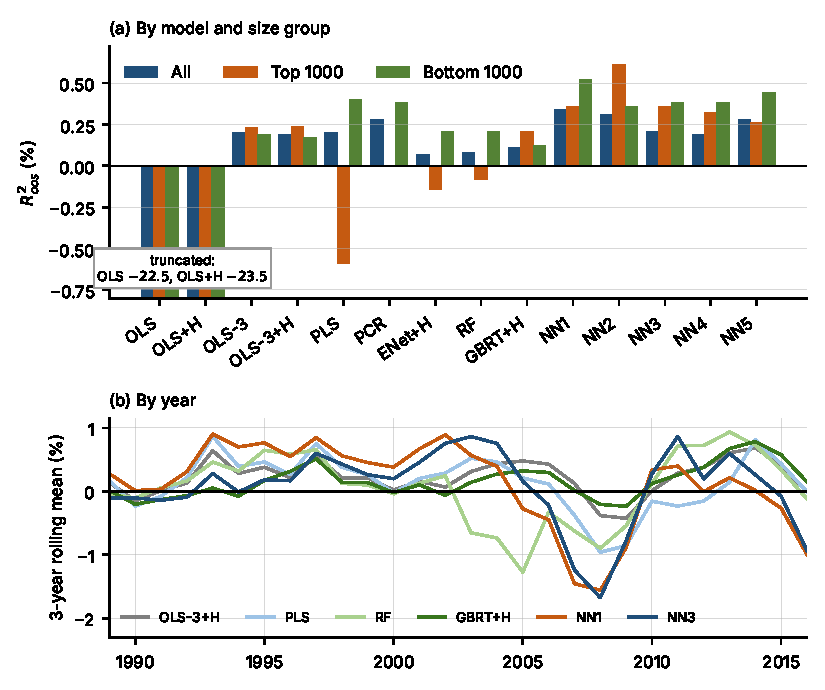
\includegraphics[width=\linewidth]{figures/fig_r2.pdf}
\caption{Out-of-sample $R^2$. (a) All stocks and the 1,000 largest / smallest stocks; OLS and OLS+H are truncated.
(b) Three-year rolling mean of annual $R^2_{oos}$ for selected models.}\label{fig:r2}
\end{figure}

\subsection{Q2: Linear models -- overfitting, robust loss, regularisation}
With 920 inputs, OLS and OLS+H reach $-22.5\%$ and $-23.5\%$ and are positive in only 2 and 1 of 30 years. The sign matches
GKX but the magnitude is much larger. The losses come from a small set of explosive forecasts: the standard deviation of
OLS forecasts is 9\% per month (PLS: 1.1\%), about 15\% of forecasts exceed $\pm10\%$ per month, and capping forecasts at
$\pm5\%$ would give $-3.25\%$ (a diagnostic, not a result we report as ours). They arise from nearly collinear inputs: a
characteristic and its interactions with slowly moving macro predictors, and near-duplicate characteristic pairs such as
\texttt{beta}/\texttt{betasq} and \texttt{pchsaleinv}/\texttt{pchsale\_pchinvt}. These four characteristics carry 71\% of the
variable importance of OLS+H, i.e.\ the fit relies on large offsetting coefficients that stop offsetting when the inputs
leave their training range. The damage is largest in the first test years (1987: $-177\%$), when the training window is
shortest and macro predictors vary least. The Huber loss does not help (OLS+H is not more accurate than OLS; DM $-1.26$),
because it limits the influence of extreme \emph{returns} in training, while the problem is extrapolation in the
\emph{inputs}. We cannot fully exclude that single-precision Gram-matrix products on the GPU amplified the instability,
and the data vintage is a further source of difference; neither changes the conclusion that unregularised OLS is by far the
worst model.

Shrinkage and dimension reduction restore positive predictability (ENet+H 0.07\%, PCR 0.28\%, PLS 0.20\%), but they only
match the three-characteristic benchmark. Figure~\ref{fig:complex} shows how little of the input space they use. The elastic
net keeps 0--1 coefficients from 1988 to 1998, i.e.\ it essentially forecasts a constant, and 45--215 after 2000. PCR uses
30--50 components until 2011 and 5--15 in most later years, and PLS uses 1--3 components in most years and 9--11 in 2005--2011.
As in GKX's Figure~3, the linear signal is low-dimensional and models become more complex only as the training sample
grows.

\begin{figure}[t]\centering
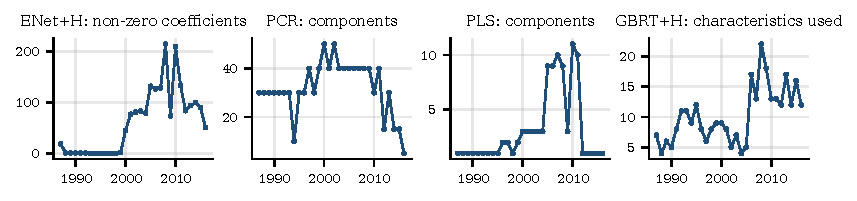
\includegraphics[width=\linewidth]{figures/fig_complexity.pdf}
\caption{Model complexity selected at each annual refit, 1987--2016.}\label{fig:complex}
\end{figure}

\subsection{Q3: Nonlinear models and how macro information should enter}\label{sec:nonlinear}
\paragraph{Trees.} Our first tree specification gave the trees the 94 characteristics \emph{and} the 8 macro predictors as
standalone levels. Both models then lost out of sample (RF $-0.66\%$, GBRT+H $-0.11\%$). A decomposition of the forecasts
shows why: the dispersion over time of the monthly \emph{average} forecast was six to seven times the dispersion of
forecasts across stocks within a month (RF: 0.0166 vs.\ 0.0024), whereas for the networks it is about one fifth. The trees
had used the macro levels to forecast the common, market-wide component of returns, which is dominated by noise (RF lost
10.6\% in 2003 alone); keeping only the cross-sectional part of the same forecasts gives $+0.15\%$ and $+0.14\%$. In GKX,
macro predictors enter only through interactions with centred characteristics, so they cannot shift all forecasts together.
Removing the standalone levels -- our final specification -- restores positive $R^2_{oos}$ (RF 0.08\%, GBRT+H 0.11\%) and
reduces the time-series dispersion of the average forecast to the level of the cross-sectional one. The trees remain below
GKX (0.33\%, 0.34\%), because they now see no macro information at all; an independent implementation that feeds the trees
all 920 interaction terms gives 0.24\% and 0.19\%. The lesson is that a flexible model given macro levels can learn
market timing, a much harder problem than ranking stocks, and that GKX's interaction design is not innocuous.

\paragraph{Networks.} The networks are the best family. Performance peaks at the shallowest architectures (NN1 0.34\%, NN2
0.31\%) and does not improve with depth (NN3--NN5 0.19--0.28\%), in line with GKX's ``shallow learning'' finding that a few
hidden layers capture the useful nonlinearity in a low signal-to-noise problem. The ranking among NN1--NN5 is not
statistically meaningful (all pairwise DM statistics $|t|<1.4$, Table~\ref{tab:dm}), and the year-by-year $R^2$ of the five
networks are highly correlated (0.77--0.96): they agree on \emph{when} returns are predictable.

\begin{table}[t]\centering\scriptsize\setlength{\tabcolsep}{3.2pt}
\caption{Diebold--Mariano statistics, 1987--2016. Positive: the column model is more accurate than the row model.
$|DM|>1.96$: 5\% level (bold); $|DM|>2.64$: Bonferroni-adjusted for 12 comparisons, as in GKX.}\label{tab:dm}
\begin{tabular}{lrrrrrrrrrrr}\toprule
 & OLS-3+H & PLS & PCR & ENet+H & RF & GBRT+H & NN1 & NN2 & NN3 & NN4 & NN5 \\\midrule
OLS+H   & \textbf{4.24} & \textbf{4.23} & \textbf{4.25} & \textbf{4.28} & \textbf{4.20} & \textbf{4.22} & \textbf{4.25} & \textbf{4.26} & \textbf{4.26} & \textbf{4.26} & \textbf{4.27} \\
OLS-3+H &  & 0.03 & \textbf{2.53} & $-0.99$ & $-0.92$ & $-1.64$ & 0.97 & 1.09 & 0.04 & $-0.02$ & 1.03 \\
PLS     &  &  & 1.77 & $-0.95$ & $-0.88$ & $-0.92$ & 1.17 & 1.18 & 0.03 & $-0.04$ & 0.95 \\
PCR     &  &  &  & $-1.59$ & $-1.67$ & $\mathbf{-2.45}$ & 0.19 & 0.18 & $-0.48$ & $-0.61$ & 0.01 \\
ENet+H  &  &  &  &  & 0.05 & 0.30 & 1.53 & \textbf{2.03} & 0.89 & 0.87 & 1.82 \\
RF      &  &  &  &  &  & 0.25 & 1.64 & 1.44 & 0.63 & 0.60 & 1.21 \\
GBRT+H  &  &  &  &  &  &  & 1.48 & 1.71 & 0.52 & 0.52 & 1.81 \\
NN1     &  &  &  &  &  &  &  & $-0.01$ & $-0.85$ & $-1.07$ & $-0.18$ \\
NN2     &  &  &  &  &  &  &  &  & $-1.11$ & $-1.37$ & $-0.25$ \\
NN3     &  &  &  &  &  &  &  &  &  & $-0.14$ & 0.66 \\
NN4     &  &  &  &  &  &  &  &  &  &  & 0.89 \\
\bottomrule\end{tabular}
\end{table}

\paragraph{Statistical significance.} Every other model in Table~\ref{tab:dm} is significantly more accurate than OLS+H (DM $\approx4.2$, surviving the
Bonferroni correction). Beyond that, only three comparisons are significant at 5\% (PCR over OLS-3+H and over GBRT+H, NN2
over ENet+H), and none survives the Bonferroni threshold. The networks are numerically ahead of most linear models (positive
DM statistics in the ENet+H, RF and GBRT+H rows) but not significantly so. Our separation between the better models is
therefore weaker than in GKX; smaller ensembles, coarser tuning and the public data release all add noise to forecasts whose
differences are small relative to the noise in returns.

\subsection{Q4: Which predictors matter?}
\begin{figure}[t]\centering
\begin{minipage}[c]{0.55\linewidth}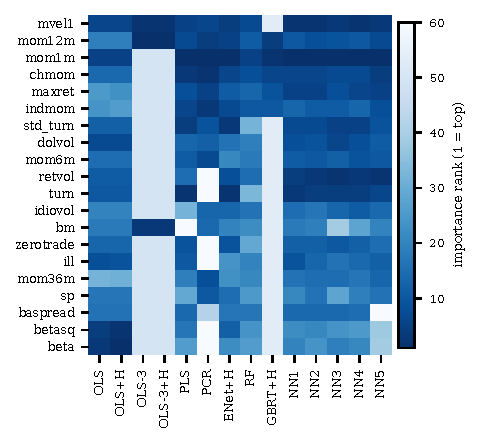
\includegraphics[width=\linewidth]{figures/fig_vi.pdf}\end{minipage}\hfill
\begin{minipage}[c]{0.42\linewidth}\scriptsize\setlength{\tabcolsep}{2.5pt}
\begin{tabular}{lrrrrr}\toprule
 & Trend & Liquid. & Risk & Value & Other \\\midrule
OLS+H & 0.07 & 0.12 & 0.41 & 0.02 & 0.38 \\
OLS-3+H & 0.57 & 0.28 & 0.00 & 0.15 & 0.00 \\
PLS & 0.59 & 0.32 & 0.02 & 0.01 & 0.07 \\
PCR & 0.85 & 0.05 & 0.01 & 0.03 & 0.05 \\
ENet+H & 0.53 & 0.29 & 0.07 & 0.05 & 0.06 \\
RF & 0.20 & 0.09 & 0.04 & 0.05 & 0.62 \\
GBRT+H & 0.34 & 0.00 & 0.00 & 0.00 & 0.66 \\
NN1 & 0.49 & 0.37 & 0.09 & 0.02 & 0.03 \\
NN3 & 0.43 & 0.35 & 0.14 & 0.02 & 0.05 \\
NN5 & 0.54 & 0.24 & 0.12 & 0.04 & 0.07 \\
\bottomrule\end{tabular}\end{minipage}
\caption{Variable importance. Left: rank of the 20 most important characteristics in each model (darker = more important).
Right: share of importance by group -- price trend (mom1m, mom6m, mom12m, mom36m, chmom, indmom, maxret), liquidity
(mvel1, dolvol, std\_dolvol, turn, std\_turn, ill, zerotrade, baspread), risk (retvol, idiovol, beta, betasq), valuation and
fundamentals (bm, ep, sp, cfp, dy, agr, roaq, roeq, sgr, lev).}\label{fig:vi}
\end{figure}

Averaged over the 14 models, the most important characteristics are short-term reversal \texttt{mom1m} (20.8\% of total
importance), 12-month momentum \texttt{mom12m} (11.3\%), size \texttt{mvel1} (9.3\%), turnover \texttt{turn} (4.5\%), momentum
change \texttt{chmom} (4.4\%), volatility \texttt{retvol} (3.9\%), \texttt{std\_turn} (3.2\%) and \texttt{maxret} (2.9\%). This
is essentially GKX's list (Figures~4--5): all methods agree on a small set of price-trend, liquidity and volatility signals,
while valuation ratios and accounting fundamentals receive about 5\% of importance or less outside OLS-3 (Figure~\ref{fig:vi}).
Models differ in how concentrated they are: PCR puts 85\% on price trends and PLS/ENet+H 37\% on \texttt{mom1m} alone,
whereas the networks spread importance over trend (42--54\%), liquidity (24--37\%) and risk (9--14\%) -- the same contrast
GKX draw between linear and nonlinear models. Unregularised OLS+H is the outlier, dominated by the near-duplicate pairs
discussed in Q2.

Two measurement caveats matter for interpretation. (i) For the trees, binary indicators (\texttt{divi}, \texttt{divo},
\texttt{sin}, \texttt{convind}) rank high (the ``other'' column). After rank-normalisation their ``0'' group lies slightly
below zero while missing values are exactly zero, so trees can split on data availability, and setting such an input to zero
marks every stock as missing; this overstates their importance, and replacing zero by the monthly median (provided as an
option in our code) removes the artefact. (ii) Among macro predictors, PLS and ENet+H rely mainly on the T-bill rate,
default spread and aggregate book-to-market ratio, whereas the networks use almost exclusively the dividend-- and
earnings--price ratios. Because macro predictors enter the interactions in raw units (\texttt{dp}, \texttt{ep} $\approx-3$;
T-bill rate $\approx0.05$; stock variance $\approx0.002$) and the networks are trained with an L1 penalty, this partly
reflects input scale rather than economic relevance. Trees have no macro importance by construction.

\subsection{Q5: Stability and economic value}
Predictability is far from uniform over time (Figure~\ref{fig:r2}b). All models lose in 2007--2008 (networks
$-2.1\%$ to $-2.6\%$ in 2007) and recover strongly in 2009 (NN3 $+2.3\%$). The nonlinear models are positive in 17--21 of 30 years. Statistical significance and economic value also differ:
sorting stocks each month into deciles on the forecast, the long--short portfolio of NN3 earns 2.68\% per month
equal-weighted (annualised Sharpe ratio 1.81) and 1.56\% value-weighted (Sharpe 0.94), compared with 0.81 and 0.42 for
OLS-3+H and 1.59 and 0.68 for PLS. GKX report a value-weighted Sharpe ratio of 1.35 for their network strategy; our lower
figure is consistent with our smaller $R^2$ among large stocks. A monthly $R^2$ of a few tenths of a percent, applied to
thousands of stocks every month, is economically meaningful.

% =====================================================================
\section{Discussion and limitations}
(i) \emph{Compute.} Smaller ensembles, coarser tuning and biennial refits for NN2--NN4 lower and add noise to the
network results; this likely explains part of the weaker DM separation. (ii) \emph{Data.} The public 2021 release covers
fewer stocks per month than the original sample, and differences in characteristic construction may shift results.
(iii) \emph{Trees.} Our final trees see no macro information; the 920-input variant shows that adding it through
interactions helps (0.24\%/0.19\%), but it is a separate implementation and is reported only as a robustness check.
(iv) \emph{OLS.} We could not run the full OLS models in double precision on a GPU within the project; a diagnostic option
is included in our code. (v) \emph{Variable importance} is a property of the fitted model, correlated characteristics share
credit, and the zeroing convention has the caveats above. (vi) The test period is one historical path; single-year results
are noisy.

\section{Conclusion}
We reproduce GKX's central conclusions with public data: OLS with hundreds of predictors overfits catastrophically;
shrinkage and dimension reduction recover modest predictability that is low-dimensional; shallow neural networks give the
best forecasts, and depth beyond one or two hidden layers does not help; and all methods agree that short-term reversal,
momentum, size, liquidity and volatility drive expected returns. Beyond the paper, we find that the way macroeconomic
information enters a flexible model is decisive -- as standalone levels it invites market timing and out-of-sample losses --
and that, with our data and compute, most differences among the better models are not statistically significant.

% =====================================================================
\section*{Contributions}
\small
\textbf{Zhang Qi}: data pipeline (panel construction, timing check, rank normalisation, Welch--Goyal predictors), project
coordination, integration of all results (tables, DM tests, figures), code repository, report writing and slides.
\textbf{Wei Fanjing}: estimation of the seven linear models and NN1 on Kaggle GPUs, Diebold--Mariano tests and the
model-complexity analysis, draft of the linear-model results.
\textbf{Tang Yunshu}: estimation of RF, GBRT+H and NN5; diagnosis of the tree failure, the corrected tree specification and
an independent 920-input tree implementation; variable-importance analysis across all models and its draft.
\textbf{Du Yunhe}: estimation of NN2--NN4 under the reduced protocol, draft of the neural-network results and the
stability analysis, video recording and editing.

\section*{Use of AI tools}
\small
The code framework (data processing, streamed linear estimators, tree and network wrappers, recursive evaluation, metrics),
the diagnostic analyses and the drafting and editing of this report were done with the help of Claude (Anthropic). Tang
Yunshu used an LLM coding assistant to review the variable-importance code, draft analysis scripts and edit her section.
Du Yunhe used WorkBuddy to set up the environment, launch and monitor the estimation, check outputs and draft his section.
Wei Fanjing used Codex to review the results of the model-complexity analyses and to edit her report section. All code was run and checked by the team; every number in this
report is computed from the team's own forecasts with the code in the repository, and interpretations were checked against
GKX.

\section*{Code and data}
\small
Code, notebooks (including each member's executed runs), final tables and figures:
\url{https://github.com/ZQ-77777/gkx-replication}. Data: the authors' public characteristics (Dacheng Xiu's website) and
the Welch--Goyal data (Amit Goyal's website).

\begin{thebibliography}{99}\small
\bibitem{gkx} S.~Gu, B.~Kelly and D.~Xiu. Empirical asset pricing via machine learning. \emph{Review of Financial Studies}, 33(5):2223--2273, 2020.
\bibitem{wg2008} I.~Welch and A.~Goyal. A comprehensive look at the empirical performance of equity premium prediction. \emph{Review of Financial Studies}, 21(4):1455--1508, 2008.
\bibitem{huber} P.~J. Huber. Robust estimation of a location parameter. \emph{Annals of Mathematical Statistics}, 35(1):73--101, 1964.
\bibitem{zou} H.~Zou and T.~Hastie. Regularization and variable selection via the elastic net. \emph{Journal of the Royal Statistical Society B}, 67(2):301--320, 2005.
\bibitem{breiman} L.~Breiman. Random forests. \emph{Machine Learning}, 45(1):5--32, 2001.
\bibitem{friedman} J.~H. Friedman. Greedy function approximation: a gradient boosting machine. \emph{Annals of Statistics}, 29(5):1189--1232, 2001.
\bibitem{xgb} T.~Chen and C.~Guestrin. XGBoost: a scalable tree boosting system. In \emph{KDD}, pages 785--794, 2016.
\bibitem{adam} D.~P. Kingma and J.~Ba. Adam: a method for stochastic optimization. In \emph{ICLR}, 2015.
\bibitem{bn} S.~Ioffe and C.~Szegedy. Batch normalization: accelerating deep network training by reducing internal covariate shift. In \emph{ICML}, pages 448--456, 2015.
\bibitem{dm} F.~X. Diebold and R.~S. Mariano. Comparing predictive accuracy. \emph{Journal of Business \& Economic Statistics}, 13(3):253--263, 1995.
\end{thebibliography}
\end{document}
